% !TEX root = ../../../main.tex
% 来源：中学数学实验教材·第一册（代数）
% 章节：一元二次方程 / 解应用问题
% 原始文件：3.tex，行 3290-3295
% 类型：tikz
% ---
        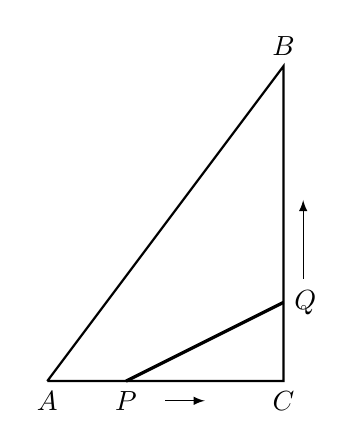
\begin{tikzpicture}[>=latex]
     \draw[thick] (0,0)node[below]{$A$}--(3,0)node[below]{$C$}--(3,4)node[above]{$B$}--(0,0) ;
     \draw[very thick] (1,0)node[below]{$P$}--(3,1)node[right]{$Q$};     
\draw [->] (1.5,-.25)--(2,-.25);
\draw [->] (3.25,1.3)--(3.25,2.3);
        \end{tikzpicture}
